%==============================================================================
%  Chapter 2 — Background and theoretical framework
%
%  Two-part structure:
%    Part A: Empirical context — the EIC, Pathfinder, STEP, the Sovereignty Seal
%    Part B: Theoretical lens   — institutional logics (primary), isomorphism,
%                                 legitimacy, three pillars (subsidiary),
%                                 mission-oriented investment / developmental
%                                 state literature
%
%  End the chapter with an explicit "analytical framework" section that bridges
%  the two parts and is referred back to in Chapters 4 and 5.
%==============================================================================
\chapter{Background and Theoretical Framework}
\label{ch:background}

\section*{Chapter overview}

The chapter has two parts. The first part places the two instruments
under study, Pathfinder and STEP Scale Up, inside the EIC's portfolio
and the wider EU innovation-policy lineage, and describes their design
at the level needed to follow the rest of the thesis. The second part
sets out the theoretical lens. Institutional logics, in the
Friedland--Alford and Thornton tradition, is treated as the primary
construct; isomorphism, legitimacy and Scott's three pillars are
brought in as complementary lenses; and the mission-oriented and
developmental-state literatures provide the comparator vocabulary
against which STEP's investment mechanics will later be read. The
chapter closes with a synthesis that names the framework Chapters
\ref{ch:results} and \ref{ch:discussion} mobilise.

%==============================================================================
\section{The EIC and its place in EU innovation policy}
\label{sec:bg-eic}

The European Innovation Council (EIC) is the most recent layer in a
long lineage of EU research and innovation funding. The Framework
Programmes have funded collaborative research since FP1 in 1984; FP7
(2007--2013) introduced the European Research Council for frontier
science; Horizon~2020 (2014--2020) added the SME Instrument and a
pilot EIC; and Horizon Europe (2021--2027) established the EIC on a
permanent footing as Pillar~III of the Programme, alongside the
Excellent Science and Global Challenges pillars
\parencite{ec2025eicwp}. The EIC's mandate is breakthrough
innovation: technologies whose risk profile is judged too high for
private capital alone, and which sit too close to market for the
research-only logic of the ERC.

The EIC operates four main instruments. \emph{Pathfinder} funds
early-stage, high-risk research at Technology Readiness Levels
(TRL)~1--4. \emph{Transition} bridges proof-of-concept to a
market-ready offer at TRL~4--6. \emph{Accelerator} funds late-stage
start-ups with blended grant-and-equity packages. The EIC also runs a
prize portfolio and a suite of business-acceleration services. Layered
on top of these instruments since 2024, the Strategic Technologies for
Europe Platform (STEP) channels additional capacity into a set of
priority technology families and adds two of its own delivery routes,
including the STEP Scale Up window inside the EIC \parencite{eu2024step}.

The thesis attends to Pathfinder and STEP Scale Up because they bracket
the EIC pipeline at its two most informative inflection points. Pathfinder
sits at the earliest stage of public risk-bearing, where the object
funded is a scientific hypothesis. STEP Scale Up sits at the
furthest reach of public capital into commercial growth, where the
object funded is a company seeking equity finance for industrial
expansion. Holding the agency, governance and Work Programme constant
across these two ends of the pipeline isolates how the textual
treatment of evidence, applicant and success shifts as the EIC moves
from underwriting science to underwriting industrial scale. Transition
and Accelerator are deliberately left out: they occupy the middle of
the pipeline, where the contrast that makes the pairing analytically
useful is muted. The reasoning is set out in
\cref{sec:meth-corpus}.

%==============================================================================
\section{The Pathfinder instrument}
\label{sec:bg-pathfinder}

Pathfinder funds research at the earliest stage of the innovation
chain. Eligible applicants are consortia of at least three independent
legal entities from three different Member States or Associated
Countries, with universities, research organisations and small
companies as the typical participants. The instrument has two
sub-streams. \emph{Pathfinder Open} is bottom-up: applicants propose
the topic and the science. \emph{Pathfinder Challenges} is top-down:
the Commission, advised by external Programme Managers, sets a small
number of thematic calls each year, and consortia apply against those
themes.

The technology readiness range is TRL~1--4, which the Work Programme
treats as the span from basic principles observed (TRL~1) to
technology validated in laboratory conditions (TRL~4). The instrument
funds grants only; there is no equity component. Budget envelopes are
set per call in the annual Work Programme, with individual awards
typically in the low millions of euro and durations of three to four
years. Evaluation runs on the EIC's adapted version of the Horizon
Europe criteria, with \emph{excellence} (including scientific novelty
and the credibility of the breakthrough claim), \emph{impact}
(including a plausible commercialisation pathway) and the
\emph{quality and efficiency of implementation}. Selection is by
remote expert review followed by an interview-style jury for Challenges.

Two features of Pathfinder's governance are relevant to the later
analysis and are noted descriptively here. The first is the role of
\emph{Programme Managers}: senior experts contracted by the EIC to
shape the Challenges, advise on portfolio composition, and act as
sparring partners to funded teams. The second is the EIC's stated
practice of \emph{active portfolio management}, by which Pathfinder
projects are followed beyond the grant agreement and steered towards
Transition, Accelerator or alternative routes. Both features are
returned to in \cref{ch:results}.

%==============================================================================
\section{STEP Scale Up and the Sovereignty Seal}
\label{sec:bg-step}

STEP was established by Regulation (EU)~2024/795 in response to the
strategic-autonomy debate of 2023--2024, which framed European
dependence in critical technologies as a sovereignty risk
\parencite{eu2024step}. The Regulation identifies three technology
families as in scope: deep and digital technologies; clean and
resource-efficient technologies; and biotechnologies. STEP does not
operate as a stand-alone fund. It is a platform: it redirects and
tops up capacity in a set of existing EU instruments, including the
EIC, the Innovation Fund, InvestEU, the European Defence Fund and
cohesion-policy programmes. Inside the EIC, STEP is delivered through
a dedicated Scale Up call that funds large equity tickets into
companies already past the early-stage phase Pathfinder addresses.

STEP Scale Up's investment mechanics differ sharply from Pathfinder's.
The instrument provides equity rather than grants, with the EIC Fund
acting as the investment vehicle on the Commission's behalf. Ticket
sizes are large by EU-instrument standards (the Work Programme cites
investments of up to \texteuro{}30~million per company, with the
Commission's stake conditioned on private co-investment). Selection
is structured around due diligence carried out by external
investment professionals, alongside the EIC's evaluation criteria.
The instrument is positioned as a catalytic anchor investor whose
participation is intended to crowd in private capital at the scale-up
stage, rather than as a buyer of last resort.

The Sovereignty Seal (formally the STEP Seal) is the device through
which STEP extends beyond the budgets it directly controls. Proposals
assessed as high quality but not funded by one STEP-eligible
instrument can be awarded the Seal and signalled to other funders, EU
and national, as endorsed targets. The Seal is therefore a portable
artefact of institutional endorsement: it circulates beyond the EIC
itself and is intended to coordinate the wider European funding
field around STEP's strategic priorities. Its design and effects are
returned to in \cref{sec:res-step-seal} and \cref{sec:disc-step-seal}.

%==============================================================================
\section{Institutional logics: the primary lens}
\label{sec:bg-it-logics}

The institutional-logics perspective begins with the claim that
society is composed of multiple, partially-incommensurable orders,
each carrying its own goods, its own measures of worth, and its own
view of who counts as a competent actor \parencite{friedland1991bringing}.
\textcite{thornton2012institutional} formalise this as an
\emph{inter-institutional system} of ideal-typical logics: the market,
the state, the corporation, the professions, religion, the family and
the community. The analytic move is to treat any concrete site, an
organisation, a field or a policy text, as the locus where one or more
of these logics is enacted, and where contradictions between them are
worked out.

Four logics are foregrounded in the present analysis because they
appear, with varying weight, across the Pathfinder and STEP texts.
The \emph{science} logic measures worth by novelty, rigour and frontier
contribution; authority sits with peer judgement; the canonical
instrument is the open competitive grant. The \emph{market} logic
measures worth by commercial viability, growth and return; authority
sits with investors and demand signals; the canonical instruments are
equity, rounds and co-investment. The \emph{state} logic measures
worth by strategic value and sovereignty; authority sits with
legislative mandate and public institutions; the canonical instruments
are regulated, conditioned and mission-tied awards. The
\emph{profession} logic measures worth by conformity with credentialled
standards; authority sits with certified specialists; the canonical
device is expert validation. A quick-reference matrix of vocabulary,
authority and instrument signatures used in coding is reproduced in
\cref{app:logics-matrix}.

Two constructs from the logics literature do most of the analytical
work in later chapters. The first is \emph{logic conflict and
hybridisation}: when two logics are simultaneously claimed in a single
site, the text either makes the conflict visible or papers it over.
The second is \emph{tension-dissolution}, the thesis's own label for
the second of these moves: a textual pattern in which logics that
should be in tension (for instance, scientific excellence and
strategic sovereignty) are presented as complementary, suppressing
visible conflict. The pattern is identified empirically in
\cref{ch:results} as Pattern~A and read theoretically in
\cref{ch:discussion} as cognitive legitimacy work in the sense of
\textcite{suchman1995managing}.

%==============================================================================
\section{Isomorphism}
\label{sec:bg-it-isomorphism}

\textcite{dimaggio1983iron}, building on \textcite{meyer1977institutionalized},
ask why organisations in a shared field come to resemble each other
even where convergence is not competitively advantageous. They
identify three mechanisms. \emph{Coercive isomorphism} operates
through formal authority: laws, mandates and the conditions attached
to funding force compliance. \emph{Mimetic isomorphism} operates under
uncertainty: actors copy models that appear successful or prestigious,
because doing so is cheaper than working out the right answer from
first principles. \emph{Normative isomorphism} operates through
professional communities: training, credentialling and inter-firm
mobility diffuse a shared repertoire of practices.

The three mechanisms map onto Scott's three pillars
(\cref{sec:bg-it-scott}) in a way that is useful to flag here:
coercive pressures produce regulative-pillar compliance; normative
pressures produce normative-pillar conformity; and mimetic pressures
operate at the cognitive pillar, where the imitated model is taken
for granted as the right shape of the problem
\parencite{scott2014institutions}.

Mimetic isomorphism is given particular weight in the later analysis,
and a note on how the mechanism is identified is warranted before the
analysis chapters. \textcite{dimaggio1983iron} characterise mimesis as
operating under uncertainty and often without conscious acknowledgement
by the imitating organisation. The diagnostic they specify is
structural resemblance to models that appear successful or prestigious
in a reference field, not textual citation of those models. Imitation
may be intentional and explicit, with the imitator naming the model
and adopting its features. It is equally often indirect, mediated
through personnel movement, consulting firms, or professional
education, and the imitator does not name the source. The three
mechanisms are therefore not textually visible in the same way:
coercive and normative pressures typically leave named traces
(regulations cited, evaluation bodies invoked, standards named);
mimetic pressures more often leave only structural traces.

The consequence for this thesis is direct. The Work Programme
benchmarks EIC performance against the USA and Asia at Strategic
Goal 4 but names no specific institutional referents. The
developmental-state literature (\cref{sec:bg-mazzucato}) supplies
DARPA \parencite{bonvillian2018darpa}, Temasek-style sovereign
investment vehicles, and the Chinese Government Guidance Funds
(\cite{li2025financing}; \cite{luong2021guidance}) as the recognised
institutional comparators for this class of state-anchor instrument.
The mimetic reading developed in \cref{sec:disc-step-mimesis} is
therefore analyst-supplied: it draws its named comparators from the
secondary literature and identifies their traces in the corpus
through structural resemblance rather than through explicit citation.

%==============================================================================
\section{Legitimacy}
\label{sec:bg-it-legitimacy}

\textcite{suchman1995managing} defines legitimacy as a generalised
perception that an entity's actions are desirable, proper or
appropriate within a socially constructed system of norms and beliefs.
The definition does three things at once. It places legitimacy in the
eye of the audience rather than in the properties of the entity; it
allows for explicit legitimation work; and it distinguishes three
sub-types. \emph{Pragmatic} legitimacy rests on the audience's
self-interest: the entity is supported because it delivers something
the audience values. \emph{Moral} legitimacy rests on normative
endorsement: the entity is supported because what it does is judged
right. \emph{Cognitive} legitimacy rests on taken-for-grantedness: the
entity is supported because no alternative is readily imagined.

The three sub-types are used asymmetrically in the analysis. Pragmatic
legitimacy is the easy register the Work Programme reaches for when it
addresses applicants and co-investors: STEP is presented as a route to
capital, a Seal as a route to follow-on funding. Moral legitimacy
underwrites the strategic-autonomy framing of STEP, in which European
sovereignty is treated as a good in itself. Cognitive legitimacy is
the most consequential for the thesis: it is the register in which
tension-dissolution operates, because the dissolution succeeds
precisely when the reader does not notice that two logics have been
made to coexist. The Sovereignty Seal is read in \cref{ch:discussion}
as a portable legitimacy artefact: a device that detaches institutional
endorsement from the funding decision and lets it circulate.

%==============================================================================
\section{Scott's three pillars}
\label{sec:bg-it-scott}

\textcite{scott2014institutions} organises the institutional
literature into three pillars, each with its own basis of compliance,
its own logic of legitimacy and its own indicators. The
\emph{regulative} pillar covers rules, monitoring and sanctioning;
compliance is expedient, and legitimacy follows from being legally
sanctioned. The \emph{normative} pillar covers values and role
expectations; compliance is appropriate, and legitimacy follows from
being morally governed. The \emph{cognitive} pillar covers taken-for-granted
schemas and shared categories; compliance is taken for granted, and
legitimacy follows from being culturally supported.

The three pillars are treated in this thesis as a subsidiary lens,
used to articulate two specific moves the empirical chapters return
to. First, the TRL scale is read as a cognitive-pillar device: a
classification so taken for granted that it carries the linear
science-to-market assumption into every passage in which it appears.
Second, the Programme Manager role is read as a soft regulative-pillar
device: an authority that shapes Pathfinder portfolios through advice
and steering rather than through formal rule-making, but whose
recommendations are routinely deferred to. Both moves are developed in
\cref{ch:results}.

%==============================================================================
\section{Mission-oriented investment and the developmental state}
\label{sec:bg-mazzucato}

Institutional theory describes how logics are enacted and contested,
but it is largely silent on the specific question of \emph{state-led
investment} as a form. For that, the thesis draws on a complementary
literature on the entrepreneurial and developmental state. The point
of departure is \textcite{mazzucato2013entrepreneurial}, which argues that the
state has historically acted as risk-taker and market-maker in the
sectors private capital has been unable or unwilling to enter, from
the internet to mRNA platforms. Mission-oriented investment in this
tradition is patient: it accepts long horizons, tolerates failure
across a portfolio, and pursues directional goals rather than
generic productivity gains. The state on this account does not
merely correct market failure; it shapes the market it then operates
in.

A second strand, on developmental-state financial statecraft and the
specific instrument of the Government Guidance Fund (GGF), gives the
comparator vocabulary that STEP's mechanics most directly invite. GGFs
combine public anchor positions with private co-investment in
state-prioritised technology areas, route capital through
quasi-independent fund managers, and use the public stake as a
crowding-in signal rather than as a buyer of last resort. The
literature on Chinese GGFs develops this design at length, both as a
mode of neo-developmental financial statecraft
\parencite{li2025financing} and through empirical assessment of the
funds' design, performance and pathologies
\parencite{luong2021guidance}. The point for the present chapter is
not to adjudicate the European case against the Chinese comparator,
but to flag that STEP's anchor-investor design, equity-only mechanics,
and strategic-technology scope are recognisable in this comparative
literature and will be read against it in
\cref{sec:disc-step}.

Two constructs from this literature do most of the work later.
\emph{Patient capital} names the time horizon and risk appetite that
distinguish state investment of this kind from conventional venture
finance. The \emph{state as market-maker} names the move by which a
state instrument creates the market signal it then claims to respond
to: by selecting a technology family, anchoring a round, and
endorsing follow-on funders, it constitutes the field of investible
opportunities. Both constructs are mobilised in
\cref{sec:disc-step-circular} to read STEP's circular market
validation, in which the public actor produces the signal it then
requires.

%==============================================================================
\section{Synthesis: an analytical framework}
\label{sec:bg-framework}

The framework that organises the empirical chapters can now be stated
compactly. The corpus is read for four institutional logics (science,
market, state, profession), tracked at the level of vocabulary,
authority and instrument signature. Where two logics are simultaneously
present, the reading attends to whether the text makes the tension
visible or dissolves it; tension-dissolution is treated as cognitive
legitimacy work, and the Sovereignty Seal is treated as a portable
legitimacy artefact. Isomorphic mechanisms are read into the design
moves the text inscribes: TRL thresholds and the STEP Regulation as
coercive; DARPA, Temasek and the Government Guidance Fund as
analyst-supplied mimetic comparators drawn from the developmental-state
literature, identified in the corpus through structural resemblance;
the freedom-to-operate analysis and the business-plan format as
normative. Scott's three pillars are used selectively to
articulate the TRL scale as a cognitive-pillar device and Programme
Manager authority as a soft regulative-pillar device. The
developmental-state literature provides the comparator vocabulary for
STEP's investment mechanics, in particular patient capital and the
state-as-market-maker.

The framework is deliberately layered rather than monolithic. Logics
do the heaviest analytical work: they identify what is being claimed
in a given passage and what is being suppressed. Isomorphism explains
why the EIC's instruments take the shapes they do at the field level.
Legitimacy explains how the co-presence of logics is held together for
an audience. The three pillars and the developmental-state literature
sit alongside as targeted complements, mobilised where they earn
their place.

\begin{figure}[H]
    \centering
    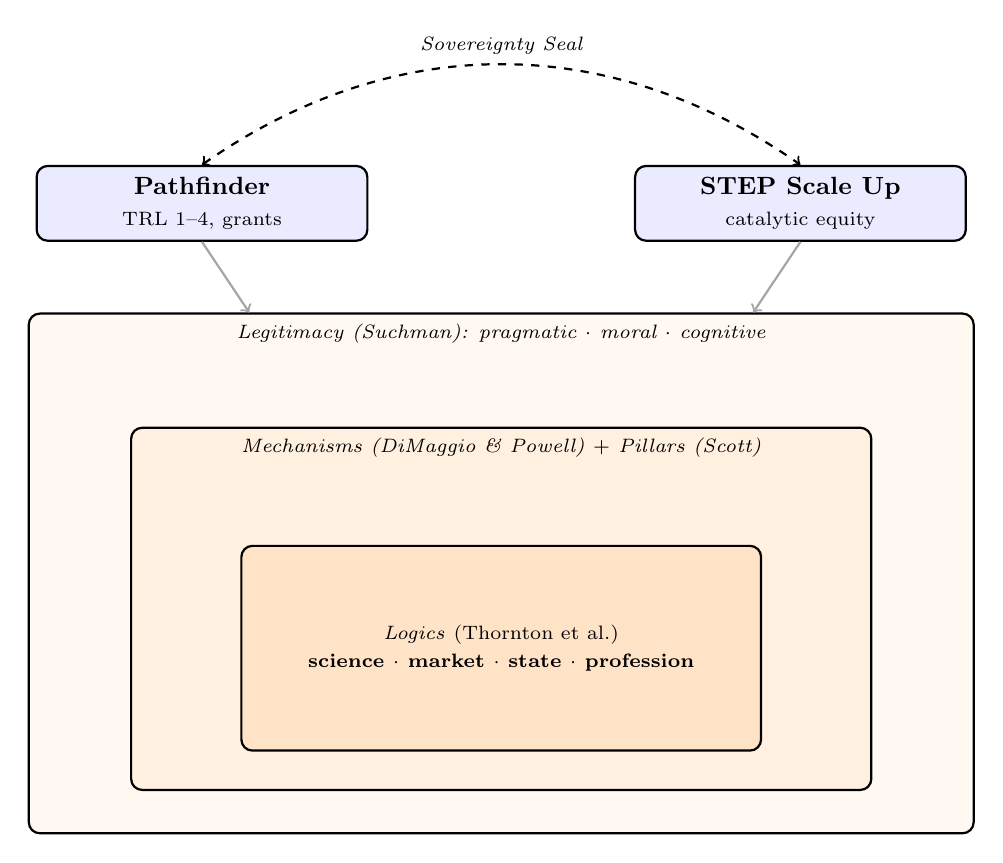
\begin{tikzpicture}[
        every node/.style={align=center},
        instrument/.style={draw, thick, fill=blue!8, rounded corners,
                           minimum width=4.2cm, minimum height=0.95cm,
                           font=\small},
        band/.style={draw, thick, rounded corners},
    ]

    % --- Three concentric analytical bands (outer to inner) ---------------
    \node[band, fill=orange!5,  minimum width=12.0cm,
          minimum height=6.6cm] (outer)  at (0,0) {};
    \node[band, fill=orange!12, minimum width=9.4cm,
          minimum height=4.6cm] (middle) at (0,-0.45) {};
    \node[band, fill=orange!22, minimum width=6.6cm,
          minimum height=2.6cm] (inner)  at (0,-0.95) {};

    % Band labels — sit in the annular margin at the top of each band
    \node[anchor=north, font=\scriptsize\itshape, inner sep=4pt]
        at (outer.north)
        {Legitimacy (Suchman): pragmatic $\cdot$ moral $\cdot$ cognitive};
    \node[anchor=north, font=\scriptsize\itshape, inner sep=4pt]
        at (middle.north)
        {Mechanisms (DiMaggio \& Powell) $+$ Pillars (Scott)};
    \node[font=\scriptsize] at (inner.center)
        {\textit{Logics} (Thornton et al.)\\[2pt]
         \textbf{science $\cdot$ market $\cdot$ state $\cdot$ profession}};

    % --- Two instrument columns above the bands ---------------------------
    \node[instrument] (pf)   at (-3.8, 4.7)
        {\textbf{Pathfinder}\\\scriptsize TRL 1--4, grants};
    \node[instrument] (step) at ( 3.8, 4.7)
        {\textbf{STEP Scale Up}\\\scriptsize catalytic equity};

    % --- Sovereignty Seal: bridging arc above the columns -----------------
    \draw[<->, thick, dashed] (pf.north) to[bend left=35]
        node[above, midway, font=\scriptsize\itshape]
        {Sovereignty Seal}
        (step.north);

    % --- Connectors from each instrument into the outer band --------------
    \draw[->, thick, gray!70] (pf.south)
        -- ([xshift=-3.2cm]outer.north);
    \draw[->, thick, gray!70] (step.south)
        -- ([xshift= 3.2cm]outer.north);

    \end{tikzpicture}
    \caption[Analytical framework]{Analytical framework guiding the
    empirical analysis. Three concentric analytical bands --- logics
    (Thornton et al.), mechanisms and pillars (DiMaggio \& Powell;
    Scott), and legitimacy types (Suchman) --- are intersected by the
    two EIC instruments under study, Pathfinder and STEP Scale Up. The
    Sovereignty Seal is drawn as a bridging artefact between the two
    instruments.}
    \label{fig:analytical-framework}
\end{figure}

\section{Chapter summary}
\label{sec:bg-summary}

The chapter has located Pathfinder and STEP Scale Up inside the EIC
portfolio and the wider Horizon Europe architecture, and has described
the two instruments at the level of design needed to follow the rest
of the thesis. It has set out the theoretical lens in layered form:
institutional logics as the primary construct, with isomorphism,
legitimacy, the three pillars and the developmental-state literature
brought in as complements. The synthesis names the framework that
\cref{ch:results} mobilises in coding the Work Programme and that
\cref{ch:discussion} returns to in interpreting the patterns.
\Cref{ch:methodology} sets out the research design, the three-pass
analytical procedure and the quality criteria that frame what the
study can and cannot claim from this framework.
